%------------------------------------------------------------------------------
% Template file for the submission of papers to IUCr journals in LaTeX2e
% using the iucr document class
% Copyright 1999-2012 International Union of Crystallography
% Version 1.5 (7 March 2012)
%------------------------------------------------------------------------------

\documentclass[pdf]{iucr}

\usepackage{bbold}
\usepackage{amsmath}
\usepackage{refstyle}
\newref{eqn}{%
name={eqn~},
names={eqns~},
Name={Eqn~},
Names={Eqns~},
rngtxt={\ to~},
lsttxt={\ and~},
refcmd=(\ref{#1})
}
\newref{fig}{%
name={fig~},
names={figs~},
Name={Fig~},
Names={Figs~},
rngtxt={\ to~},
lsttxt={\ and~},
refcmd=(\ref{#1})
}
\newref{sec}{%
name={section~},
names={sections~},
Name={Section~},
Names={Sections~},
rngtxt={\ to~},
lsttxt={\ and~},
refcmd=\ref{#1}
}
\usepackage{tikz}
\usepackage{cctbx_notations}


\journalcode{A}           % Indicate the journal to which submitted
                                  %   A - Acta Crystallographica Section A
                                  %   B - Acta Crystallographica Section B
                                  %   C - Acta Crystallographica Section C
                                  %   D - Acta Crystallographica Section D
                                  %   E - Acta Crystallographica Section E
                                  %   F - Acta Crystallographica Section F
                                  %   J - Journal of Applied Crystallography
                                  %   S - Journal of Synchrotron Radiation

\begin{document}

\newcommand{\olexrefine}{Olex2 refine}

\title{The Olex2 refinement engine}
\shorttitle{\olexrefine}  % Abbreviated title for use in running heads

     % Authors' names and addresses. Use \cauthor for the main (contact) author.
     % Use \author for all other authors. Use \aff for authors' affiliations.
     % Use lower-case letters in square brackets to link authors to their
     % affiliations; if there is only one affiliation address, remove the [a].

\newcommand{\brukerfr}{Bruker AXS-SAS, 4 Allée Lorentz, 77447 Marne-la-Vallée cedex 2, \country{France}}
\newcommand{\durhamchem}{Chemistry Department, Durham University, South Road, Durham, DH1~3LE, \country{UK}}
\newcommand{\olexsys}{OlexSys Ltd, \durhamchem}
\newcommand{\cci}{CCI, Lawrence Berkeley Laboratory, 1 Cyclotron Road, BLDG 64R0121, Berkeley, CA 94720-8235, \country{USA}}

\cauthor{Luc J.}{Bourhis}{luc\_j\_bourhis@mac.com}{\brukerfr}
\author{Oleg V.}{Dolomanov}
\author{Richard J.}{Gildea}
\author{Judith A. K.}{Howard}
\author{Horst}{Puschmann}

\aff{\durhamchem}

\shortauthor{Bourhis, Dolomanov, Gildea, Howard and Puschmann} % abbreviated author list for use in running heads

\keyword{small molecules}\keyword{refinement}\keyword{constraints}\keyword{restraints}\keyword{least-squares}

\maketitle

\begin{synopsis}
Supply a synopsis of the paper for inclusion in the Table of Contents.
\end{synopsis}

\begin{abstract}
Abstract goes here.
\end{abstract}

\section{Introduction}
\label{sec:introduction}

Almost all crystallographic computing routinely routinely carried out in Small-Molecule crystallography utilises software produced by just one author: George Sheldrick. His excellent programs, -- collectively known as ShelX -- are tried, tested and trusted by the crystallographic community.  Furthermore, ShelX has been actively developed by the eminent author over the last 40 years, with the latest version of the refinement program ShelXL about to be released in early 2013.

From a certain point of view, the field of small-molecule crystallography has reached maturity and no longer in need of further development. The fact that further development has happened, both within ShelX as well as in the many other groups that are actively developing software in this area is telling, though. Not all needs of the Small-Molecule crystallographer are adequately addressed by ShelX, and many small programs exist carrying out highly specialised taks. A retro-fit integration of many of these tasks into ShelX may well be desirable, but is unlikely to ever happen. Firstly, the code-base of ShelX is truly excellent in its brevity, but impenetrable to most. Secondly -- and more importantly -- the whole `philosophy' of ShelX is that of a `One-Man-Show'.  It is simply inconceivable that the stability and success of ShelX should be threatened by the whimsical addition of functionality by outsiders.

When we first embarked on the project reported herein, we were very clear about one point: We wanted to create a new and flexible refinement engine in a collaborative effort, based on a trusted and mature pre-existing code-base. This refinement engine would be open-source and open for inspection as well as modification by anyone. Modern programming paradigms unheard of when most crystallographic software was born, would be adhered to with the effect that extensions will always be possible and will not endanger the underlying functionality.


\section{Constraints}
\label{sec:constraints}

Constraints may be conceptualised mainly in two manners, that we will first illustrate on a simple example, a geometrically constrained acetylenic hydrogen, $C' \equiv C - H$. The position of the hydrogen must be such that the distance CH is equal to some ideal bond length $d$ and such that the angle $\widehat{C'CH}$ is equal to $180^\circ$. Expressed in such an implicit manner, those restrictions could be used to construct restraints by adding to the function to minimise a term $w_1 (CH - d)^2 + w_2 (\cos \widehat{C'CH} - 1)^2 + w_3 (\sin  \widehat{C'CH})^2$. By doing so, the number of refined parameters would not be changed but the number of observations would increase by three. 

It is however traditional to do the opposite, by reducing the number of parameters by 3 and keeping the number of observations unchanged. This is achieved by using the implicit form of the constraints to express the position of $H$ as a function of the positions of the two carbon atoms. Denoting by $x$ the triplet of coordinates of the atoms,
\begin{equation}
x_H = x_C + d \frac{x_C - x_{C'}}{\norm{x_C - x_{C'}}},
\end{equation} 
where $\norm{.}$ denotes the Euclidean norm. By using this formula, the observable $Y_c$ of the fit (either $\modulus{F_c}^2$ or $\modulus{F_c}$) that used to depend on $x_C$, $x_{C'}$ and $x_H$ is replaced by a function $\tilde{Y}_c$ of $x_C$ and $x_{C'}$ but not of $x_H$. We will call this transformation a reparametrisation: $\tilde{Y}_c(x_C, x_{C'}) = Y_c(x_C, x_{C'}, x_H(x_C, x_{C'}))$. The derivatives for the remaining variables are then obtained with the chain rule\footnote{For a column vector $x=(x_1, x_2, x_3)$, $\partialder{F}{x}$ will always denote the row vector $\left(\partialder{F}{x_1}, \partialder{F}{x_2}, \partialder{F}{x_3}\right)$. Given another column vector $y=(y_1, y_2, y_3)$, $\partialder{y}{x}$ will always denote the matrix $\left(\partialder{y_i}{x_j}\right)_{1 \le i,j \le 3}$ where $i$ (resp. $j$) indexes the rows (resp. the columns). The identity matrix will be denoted by $\identity$.},
\begin{align}
\partialder{\tilde{Y_c}}{x_C} &= \partialder{Y_c}{x_C} + \partialder{Y_c}{x_H} \partialder{x_H}{x_C}, \\
\partialder{\tilde{Y_c}}{x_{C'}} &= \partialder{Y_c}{x_{C'}} + \partialder{Y_c}{x_H} \partialder{x_H}{x_{C'}}. \nonumber
\end{align}
It should be noted that it is customary to work within the ``riding" approximation,
\begin{align}
\partialder{x_H}{x_{C'}} = 0,\ \partialder{x_H}{x_C} = \identity,
\end{align} 
which results in the much simplified chain rule
\begin{align}
\partialder{\tilde{Y}_c}{x_C} &= \partialder{Y_c}{x_C} + \partialder{Y}{x_H}, \\
\partialder{\tilde{Y}_c}{x_{C'}} &= \partialder{Y_c}{x_{C'}}, \nonumber
\end{align}
implemented in all refinement programs, including Olex2.

It is not always the case that all three coordinates of an atom are removed from the refinement by constraints. For example, an atom on the plane of the mirror $z,y,x$ has its coordinates $(x_1, x_2, x_3)$ constrained by the relation $x_1 = x_3$. The corresponding reparametrisation reads
\begin{align}
x_1 = u,\ x_2 = v,\ x_3 = u,
\label{eqn:specialposexamplereparam}
\end{align}
the observable $Y_c$ becoming now a function of the refinable parameters $(u,v)$.

In other cases, a reparametrisation will make some crystallographic parameters disappear while introducing new refinable parameters. A typical example is that of a tetrahedral $C' - CH_3$ as the geometrical constraints leave one degree of freedom, a rotation about the axis $C' - C$. Thus the reparametrisation expresses the coordinates of the hydrogen atoms $H_0$, $H_1$ and $H_2$ as functions of the coordinates of the carbon atoms, and of an angle $\phi$ modelling that rotation,
\newcommand{\hydrogenphiarg}{\!\left(\phi\!+\!n \frac{2\pi}{3}\right)}
\begin{equation}
\begin{split}
x_{H_n} = x_C 
+ d \Biggl[ &\sin \alpha \left\{ \cos\hydrogenphiarg e_1 + \sin\hydrogenphiarg e_2 \right\}\\
- &\cos\alpha e_0
\Biggr],
\end{split}
\label{eqn:rotatingch3reparam}
\end{equation}
where $\alpha \approx 109.5^\circ$ and $(e_0, e_1, e_2)$ is an orthonormal basis of column vectors with $e_0$ in the direction of the bond $C' \rightarrow C$. The riding approximation in this case consists in neglecting the derivatives of those base vectors, leading to
\begin{align}
\partialder{\tilde{Y}_c}{x_C} &= \partialder{Y_c}{x_C} + \partialder{Y_c}{x_H},\\
\partialder{\tilde{Y}_c}{\phi} &= \partialder{Y_c}{x_H} 
d \sin \alpha \left\{ -\sin\hydrogenphiarg e_1 + \cos\hydrogenphiarg e_2 \right\}.
\end{align}
Thus a new derivative with respect to the new refinable parameter $\phi$ is introduced by this reparametrisation.

The last important concept is that of the chaining or composition of reparametrisations, that we will again illustrate with a combination of the examples above. In the $CH_3$ case, the atoms $C$ and $C'$ could be on the special position studied in the next-to-last example. One way to model the hydrogen atoms in that case would be to first apply the reparametrisation \eqnref[name=]{rotatingch3reparam} and then to reparametrise $x_C$ and $x_{C'}$ using \eqnref{specialposexamplereparam}, introducing parameters $(u,v)$ for the former and $(u',v')$ for the latter. The derivatives would then be obtained by the chain rule, e.g.
\begin{equation}
\partialder{x_{H_0}}{u} = \partialder{x_{H_0}}{x_C}\partialder{x_C}{u} = 2
\end{equation}
in the riding approximation. This composition of reparametrisation is represented as a graph in the smtbx code: each parameter (some of them are triples of coordinates, others are scalars), $x_{H_0}$, $x_{H_1}$, $x_{H_2}$, $x_C$, $x_{C'}$, $\phi$, $u$, $v$, $u'$, and $v'$, constitutes a node of that graph, whereas edges are drawn from each node to the nodes it depends upon, as shown on \figref{dependencegraphexample}. 

\begin{figure}
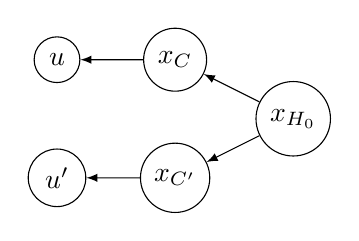
\begin{tikzpicture}[grow=left, every node/.style={circle,draw}, edge from parent/.style={-latex,draw}]
\node{$x_{H_0}$} child { node{$x_C$}    child { node{$u$}  } }
                           child { node{$x_{C'}$} child { node{$u'$} } };
\end{tikzpicture}
\label{fig:dependencegraphexample}
\caption{Example of dependency graph for the chain of reparametrisation discussed in \secref{constraints}. Only the part for hydrogen atom $H_0$ is shown.}
\end{figure}

A crystallographic refinement may involve many such reparametrisations. By piecing them all together, we obtain one reparametrisation that expresses all refinable crystallographic parameters as a smaller vector of independent parameters that shall then be refined. This piecewise construction

\appendix
\section{Computation of structure factors and their gradient}

The formulae discussed in this appendix have been known for nearly a century and have been implemented in all known refinement programs. However it seems to the authors that, during the last decades, the computation for a given Miller index~$h$ of $F_c(h)$ and its gradient $\grad{F_c(h)}$ with respect to crystallographic parameters has very rarely been presented in all the minute details necessary to implement those formulae in a program, which justifies this appendix in our humble opinion.

\subsection{Scattering factor of one atom}

\newcommand{\Fuc}{F_{\text{uc}}}

Since the structure factor of the entire unit cell is the sum over the contribution of each scatterer, we will focus on one such contribution only. We therefore consider a scatterer with  fractional coordinates $x$, a thermal displacement tensor $U^*$ in fractional coordinates and a chemical occupancy $s$ (i.e. this occupancy does not take crystallographic symmetries into account).  Its contribution $\Fuc(h)$ to the entire unit cell is obtained from its  structure factor $F(h)$  by the sum
\begin{equation}
\Fuc(h) = \sum_{\sym{R}{t} \in \cal{O}} F^{\sym{R}{t}}(h).
\end{equation}
$\cal{O}$ denotes the subset of symmetry operators $\sym{R}{t}$ of rotational part $R$ and translational part $t$ that generate the orbit of the position $x$ under the application of the entire set of symmetries in the space group of the structure whereas $F^{\sym{R}{t}}(h)$ is the transform of $F(h)$ under the symmetry $\sym{R}{t}$. For a spherical atomic model with an elastic scattering factor $f(h^2)$ that does not depend on the direction of $h$ and an inelastic scattering factor $f' + if''$ that does not depend on~$h$ (a property that holds for X-ray diffraction), $F$ reads\footnote{We will consistently denote a triplet $h$ of Miller indices as a row vector, whose transpose $h^T$ is therefore a column vector, and a triplet $x$ of fractional coordinates as a column vector. In this context, $h^2$ denotes the Euclidean square of $h$, that therefore involves the reciprocal metric matrix $M^*$ as $h^2 = h M^* h^T$.}

\begin{equation}
F(h) = s (f(h^2) + f' + i f'') \underbrace{e^{h U^* h^T} e^{i 2\pi h x}}_{G(h)}.
\end{equation}

If the thermal displacement is isotropic, the term $e^{h U^* h^T}$ is replaced by $e^{-2\pi^2 h^2 \uiso}$ and it is then factored out of $G(h)$.

We are therefore left with computing the sum of the transforms of $G(h)$ under the symmetries in $\cal{O}$, the other terms forming a factor multiplying this sum. By the definition of a Fourier transform, that transform reads
\begin{equation}
G^{\sym{R}{t}}(h) = G(hR)e^{i 2\pi ht}
\label{eqn:transformofG}
\end{equation}
Let us consider the case of centred space group first. The sum can be partioned as follow
\begin{align}
 \sum_{\sym{R}{t} \in \cal{O}} G^{\sym{R}{t}}(h) &=  \sum_{\sym{R}{t} \in \cal{O'}} \sum_{\tau \in \cal{T}} G^{(R \mid t+\tau)}(h), \nonumber\\
\intertext{where $\cal{T}$ is the set of all centring translations, including zero, whereas $\cal{O'}$ is the set of ``primitive'' symmetries. Then}
G^{(R \mid t + \tau)}(h) &= G(hR) e^{i2\pi ht} e^{i2\pi h\tau}, \nonumber \\
\intertext{but $h\tau=0$ for any Miller indices $h$ by definition, and therefore denoting by $n_{\text{ltr}}$ the order of the group of lattice translations,}
\sum_{\sym{R}{t} \in \cal{O}} G^{\sym{R}{t}}(h) &= n_{\text{ltr}} \sum_{\sym{R}{t} \in \cal{O'}} G^{\sym{R}{t}}(h)
\end{align}
which shows that the centred case and the primitive case only differ by an overall multiplicative factor.

Thus we will only consider a primitive unit cell in the following. Three cases are to be considered.
\begin{enumerate}
\item The space group is non-centric. Then there is no further simplification.
\item The space group is centric and the inversion $\inversion$ may not be located at the origin. Then the sum over the symmetries may be split into the sum over the set $\cal{O}^+$ of proper symmetries and the sum over the set of  improper symmetries. Since every improper symmetry may be written as $\inversion\sym{R}{t}$ where $\sym{R}{t}$ is a proper symmetry, we have
\begin{align}
\sum_{\sym{R}{t} \in \cal{O}} G^{\sym{R}{t}} &= 
\underbrace{\sum_{\sym{R}{t} \in \cal{O^+}} G^{\sym{R}{t}} }_{\Sigma} 
+ \sum_{\sym{R}{t} \in \cal{O}^+} G^{\inversion \sym{R}{t}}, \nonumber \\
\intertext{However the product involving the inversion simplifies as 
$\inversion\sym{R}{t} = \sym{-R}{-t + t_{\bar{1}}}$ and therefore using \eqnref{transformofG},}
G^{\inversion\sym{R}{t}} &= G(-hR) e^{-i2\pi ht} e^{i2\pi h t_{\bar{1}}}, \nonumber \\
 \intertext{but then from the very definition of $G(h)$ in \eqnref{transformofG},}
 G(-hR) &= G(hR)^*, \\
 \intertext{and therefore}
 \sum_{\sym{R}{t} \in \cal{O}} G^{\sym{R}{t}} &= \Sigma + \Sigma^* e^{i2\pi h t_{\bar{1}}}.
 \label{eqn:sumofGforcentricgroups}
\end{align}

\item If $h t_{\bar{1}}=0$, which holds true for every reflection if the space group is origin centric ($t_{\bar{1}}=0$), the previous case resolves to the real part of $\Sigma$ only,
\begin{align}
 \sum_{\sym{R}{t} \in \cal{O}} G^{\sym{R}{t}} & = 2 \sum_{\sym{R}{t} \in \cal{O}^+}  e^{h R U^* (hR)^T} \cos(hRx + t).
\end{align}
The total sum over symmetries is therefore real, and its derivative will be so too, the former involving a cosine and the latter involving a sine for the derivatives with respect to $x$. 
\end{enumerate}

In order to avoid redundant computations, our code distinguishes these three cases. One piece of code handles the case of centrosymmetric space groups using only real numbers to compute $\Sigma$. Another piece of code handles the other two cases, first computing $\Sigma$ using complex number algebra and then using \eqnref{sumofGforcentricgroups} if the space group is centric and $h t_{\bar{1}} \neq 0$. Another optimisation we applied is to precompute the terms $hR$ and $e^{i2\pi t}$ appearing in \eqnref{transformofG} as well as the test for the condition $h t_{\bar{1}}=0$ before the loop over all scatterers in the asymmetric unit. In all three cases, the computation of $\cos(hRx + t)$ and $\sin(hRx + t)$ is the most costly operation. This is mitigated\footnote{Our code also provides two options to compute the sines and cosines: either by using the trigonometric functions of the standard \cpp\ library, or by using a cctbx function that interpolates between tabulated values of sines and cosines.
} by computing the structure factor and its derivatives together, as the cosine and sine then only need to be computed once for each reflection and scatterer.
This optimisation is the reason why we have written our own new code into the smtbx instead of reusing the original code in the cctbx. Indeed, in the latter, structure factors are computed separately from the derivatives, resulting in two separate loops over the reflections and the scatterers, and in sines and cosines to be computed twice. This is rather well suited to the optimisation algorithm used in the mmtbx (LBFGS) because it does not need the derivatives at every step. But it does not fit well with full-matrix least-squares, that is prevalent in small molecule crystallography.  

\subsection{Derivatives of $\modulus{F}^2$ and $\modulus{F}$}

Having computed the unit cell structure factor $F_c$ and its derivatives, we need to compute the derivatives of $\modulus{F_c}^2$ and perhaps as well $\modulus{F_c} = \sqrt{\modulus{F_c}^2}$ if performing a refinement against $F$. Since $\modulus{F_c}^2 = F_c F_c^*$ where $z^*$ denotes the complex conjugate of the complex number $z$, for any crystallographic parameter $\xi$,
\begin{align}
\partialder{\modulus{F_c}^2}{\xi} &= F_c^* \partialder{F_c}{\xi} + F_c \partialder{F_c^*}{\xi} \nonumber \\
\intertext{but since the parameter $\xi$ is always real in practice,}
\partialder{F_c^*}{\xi} &= \left( \partialder{F_c}{\xi} \right)^* \\
\intertext{and therefore}
\partialder{\modulus{F_c}^2}{\xi} &= 2\re\left( F_c^* \partialder{F_c}{\xi}\right) \\
\intertext{where $\re$ denotes the real part. Then,}
\partialder{\modulus{F_c}}{\xi} &= \frac{1}{\modulus{F_c}} \re\left( F_c^* \partialder{F_c}{\xi}\right)
\end{align}

The smtbx provides code to compute derivatives for the both of these observables. However Olex 2 only offers the choice to refine against $F^2$.

\section{Minimisation of least-squares with an overall scale factor}

The least-squares objective function used in crystallographic refinement features an overall scale factor $K$ because we do not know on which scales are the observables $Y_o(h)$ where $Y$ denotes either $F$ or $F^2$,
\begin{equation}
L = \sum_h w(h) (Y_o(h) - K Y_c(h))^2.
\end{equation}
The parameters that each $Y_c(h)$ depends upon (atomic coordinates, ADP's, sof's) will be collectively denoted as $x_1, \cdots, x_n$. Our problem is the minimisation of $L$ with respect to all of $K, x_1, \cdots, x_n$. We will  denotes that dependency as $L(x, K)$ to keep the notations more compact, where $x$ is therefore the vector of parameters $(x_1, \cdots, x_n)$. We will denote by $(x^*, K^*)$ the values of those parameters at which $L(x,K)$ reaches the minimum we are interested in.

It is very well known that the overall scale factor tends to be highly correlated to the thermal displacements. As a result, a starting value of $K$ far from $K^*$ tends to destabilise the fit and at the very least will increase the number of iterations necessary to converge to the minimum. It is however easy to compute a reasonable approximation of $K^*$. Indeed, as a function of $K$ only, keeping all the other parameters $x$ fixed, $L(x, K)$ is a second-order polynomial. Therefore it exists an analytical formula for the value of $K$ that minimises it. Using the geometrical interpretation of least-squares is the fastest manner to demonstrate this formula and it leads to the most compact formula. We therefore introduce the scalar product of two sets of observables,

\begin{align}
Y \dotprod Y' &= \sum_h w(h) Y(h) Y'(h), \\
\intertext{and the associated norm $\norm{Y}$,}
\norm{Y}^2 &= \sum_h w(h) Y(h)^2, \\
\intertext{as well as the residual vector}
r(x, K) &= Y_o - Y_c(x).
\label{eqn:lsresidualdef}
\end{align}
With those notations, $L(x, K)$ which reads
\begin{align}
L(x, K) &= \norm{r(x, K)}^2, \\
\intertext{reaches a minimum at}
\tilde{K} &= \frac{Y_c \dotprod Y_o}{\norm{Y_c}^2},
\label{eqn:tildeK}
\\
\intertext{while keeping $x$ fixed and the value at the minimum reads}
L(x, \tilde{K}) &= \norm{Y_o}^2 - \tilde{K}^2 \norm{Y_c(x)}^2.
\end{align}
We could then simply use $\tilde{K}$ as a starting value for a combined refinement of $x$ and $K$, i.e. the minimisation of $L(x, K)$ with the independent vector $(x, K)$ of parameters.

However, we chose to minimise $L(x, \tilde{K})$ instead, which is a function of $x$ only since $\tilde{K}$ is completely determined by $x$. This is a special case of a technique called separable least-squares \cite[, and references therein]{Nielsen:2000fr} that  converges to the same minimum as previously but with fewer iterations for the same cost per iteration. In order to carry out that minimisation, we first need to compute the first-order derivatives,
\begin{align}
\partialder{L(x, \tilde{K})}{x_j} &= \partialder{L}{x_j}(x, \tilde{K}),\ 1 \le j \le n, \\
\intertext{where the chain rule would normally mandate a second term $\partialder{L}{K}(x, \tilde{K})\partialder{K}{x_j}$ but it is zero because of the definition of $\tilde{K}$. In this expression,}
\partialder{L}{x_j} &= 2 r \dotprod \partialder{r}{x_j}.
\end{align}
Thus the first-order derivative is exactly the same as it would have been with an independent parameter $K$. We then need the second-order derivatives
\begin{align}
\partialderxy{L}{x_i}{x_j} &= \partialder{r}{x_i} \dotprod \partialder{r}{x_j},\ 1 \le i,j \le n
\label{eqn:gaussleastsquares}
\end{align}
where we have neglected the term $\partialderxy{r}{x_i}{x_j} \dotprod r$ because, for a well-behaved fit, the residual $r$ and its curvature are small enough that this term can safely be neglected.

Let us now build the normal equations, which are just the Newton equations 
\begin{equation}
Bs = -g
\end{equation}
for the shift $s$ of the parameter vector $x$ where $B$ is the Hessian matrix, $B_{ij} = \partialderxy{L(x, \tilde{K})}{x_i}{x_j}$ computed using the approximation of \eqnref{gaussleastsquares} and $g$ is the gradient of $L(x, \tilde{K})$. Using the definition~\eqnref[name=]{lsresidualdef} of $r$ and the expression~\eqnref[name=]{tildeK} of $\tilde{K}$, we have
\begin{align}
\partialder{r(x, \tilde{K})}{x_i} &= -\left( \tilde{K}\partialder{Y_c}{x_i} + \partialder{\tilde{K}}{x_i} Y_c \right) \\
\partialder{\tilde{K}}{x_i} &= \frac{1}{\norm{Y_c}^2}\partialder{Y_c}{x_i} \dotprod \left(Y_o - 2 \tilde{K}Y_c \right).
\end{align}
and therefore the normal matrix $B$ and the right-hand side of the normal equations $g$ reads
\begin{align}
B &= \begin{aligned}[t] \tilde{K}^2\partialder{Y_c}{x_i} \dotprod \partialder{Y_c}{x_j} 
&+ \tilde{K} \left( \partialder{\tilde{K}}{x_j}Y_c \dotprod \partialder{Y_c}{x_i}
+ \partialder{\tilde{K}}{x_i}Y_c \dotprod \partialder{Y_c}{x_j} \right) \nonumber\\
&+ \partialder{\tilde{K}}{x_i}\partialder{\tilde{K}}{x_j} \norm{Y_c}
\end{aligned}
\\
g &= - (Y_o - \tilde{K}Y_c) \dotprod \left( \tilde{K}\partialder{Y_c}{x_i} + \partialder{\tilde{K}}{x_i} Y_c \right).
\end{align}

It should be noted that the first term of $B$ would appear in exactly the same form if we had kept the scale factor $K$ as an independent parameter. Moreover terms very similar to the second and third term of $B$ would need to be computed in that case, as the normal matrix B would then have one more column and one more row which would feature those similar terms. Thus the computation cost of our unorthodox method is the same as that of the more traditional refinement of the overall scale factor along with the other crystallographic parameters. In any case, for all methods based on the normal equations, the computation time is dominated by the first term of $B$, as it scales as $O(mn^2)$ where $m$ is the number of reflections.

\ack{Acknowledgements}

This work has been funded by the EPSRC grant ``Age Concern: Crystallographic Software for the Future" (EP/C536274/1) from the British government. We wish to thank David Watkin with whom we shared this grant for his immense contribution to our understanding of crystallographic refinement. We also wish to thank all the contributors to the CCTBX library which served as a foundation and model for our work, especially its main author Ralf W. Grosse-Kunstleve whose support has been invaluable. Finally we wish to thanks Pr. George Sheldrick for many a fruitful discussion.

\referencelist[smtbx] % References using the BibTeX database smtbx.bib

\end{document}
